
\documentclass{article}
\usepackage[table]{xcolor}
\usepackage[left=2cm, right=2cm]{geometry}
\usepackage{tikz-network}
\usepackage{amsmath}

\title{Assignment 5}
\author{Christian Parker \\ CXP22004}

\begin{document}

\maketitle

\begin{enumerate}
    % Problem 1
    \item
    \begin{align*}
        E(I_{\alpha}, J_{\alpha} = 1, J_{\beta})
            &= c (I_{\alpha} - 1)^2 + \sum_{\{\beta : \alpha \sim \beta\}}{(1 - J_{\beta})^2} + C \\
            &= c (I_{\alpha} - 1)^2 + \sum_{\{\beta : \alpha \sim \beta\}}{(J_{\beta} - 1)^2} + C
    \end{align*}
    \begin{align*}
        E(I_{\alpha}, J_{\alpha} = 0, J_{\beta})
            &= c (I_{\alpha} - 0)^2 + \sum_{\{\beta : \alpha \sim \beta\}}{(0 - J_{\beta})^2} + C \\
            &= c (I_{\alpha})^2 + \sum_{\{\beta : \alpha \sim \beta\}}{(J_{\beta})^2} + C
    \end{align*}
    \begin{center}
        C represents all terms that are independent of \(J_\alpha\)
    \end{center}
    \begin{align*}
        p
            &= P(J_{\alpha} = 1 |_\alpha J) \\
            &= \frac{P(J_{\alpha} = 1,\ _\alpha J)}{P(J_{\alpha} = 1,\ _\alpha J) + P(J_{\alpha} = 0,\ _\alpha J)} \\
            &= \frac{\frac{1}{Z'} e^{\frac{-E(I_{\alpha}, J_{\alpha} = 1, J_{\beta})}{T}}}{\frac{1}{Z'} e^{\frac{-E(I_{\alpha}, J_{\alpha} = 1, J_{\beta})}{T}} + \frac{1}{Z'} e^{\frac{-E(I_{\alpha}, J_{\alpha} = 0, J_{\beta})}{T}}} \\
            &= \frac{e^{\frac{-c (I_{\alpha} - 1)^2 - \sum_{\{\beta : \alpha \sim \beta\}}{(J_{\beta} - 1)^2} - C}{T}}}{e^{\frac{-c (I_{\alpha} - 1)^2 - \sum_{\{\beta : \alpha \sim \beta\}}{(J_{\beta} - 1)^2} - C}{T}} + e^{\frac{-c (I_{\alpha})^2 - \sum_{\{\beta : \alpha \sim \beta\}}{(J_{\beta})^2} - C}{T}}} \\
            &= \frac{e^{\frac{-c (I_{\alpha} - 1)^2 - \sum_{\{\beta : \alpha \sim \beta\}}{(J_{\beta} - 1)^2}}{T}}}{e^{\frac{-c (I_{\alpha} - 1)^2 - \sum_{\{\beta : \alpha \sim \beta\}}{(J_{\beta} - 1)^2}}{T}} + e^{\frac{-c (I_{\alpha})^2 - \sum_{\{\beta : \alpha \sim \beta\}}{(J_{\beta})^2}}{T}}}
    \end{align*}

    % Problem 2
    \item
    There are two terms in the energy function E, one measures the distance between the image I and the
    segmentation J, the second measures the smoothness of J. In the simulated annealing algorithm,
    the distance term is weighted by c. Therefore, for higher c, the distance term has greater influence
    on J than the smoothness term.

    Across the values of c tested, we can see the segmentation transition from noise to an outline of a dog
    as c increases. At low values of c, when smoothness is weighted highly, the noisiness of the initial
    uniform distribution dominates. Since the distribution is uniform, the smoothness term is a coin flip
    rather than pulling the probability distribution towards the most frequent value.
    At high values of c, the noisiness is overwhelmed by the weight of the distance term. The
    probability distribution is pulled towards the input image, shrinking the distance between I and J,
    and aligning the segmentation with the image.

    % Problem 3
    \item
        \begin{enumerate}
            \item
            Residue network:

            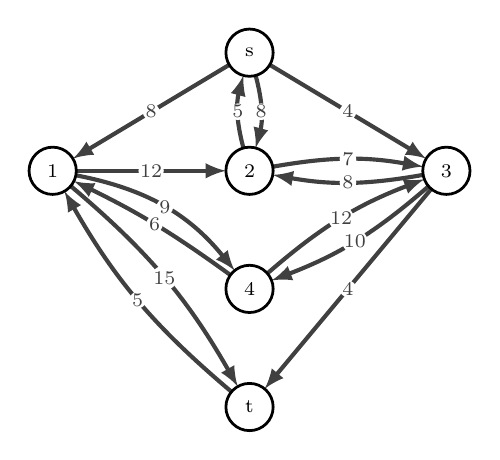
\begin{tikzpicture}[vertex/.style={fill=white}]
                \Vertex[x=2.5,y=1.5,label=s,color=white]{s}
                \Vertex[x=0,y=0,label=1,color=white]{1}
                \Vertex[x=2.5,y=0,label=2,color=white]{2}
                \Vertex[x=5,y=0,label=3,color=white]{3}
                \Vertex[x=2.5,y=-1.5,label=4,color=white]{4}
                \Vertex[x=2.5,y=-3,label=t,color=white]{t}

                \Edge[Direct,label=8](s)(1)
                \Edge[Direct,bend=15,label=8](s)(2)
                \Edge[Direct,label=4](s)(3)
                \Edge[Direct,label=12](1)(2)
                \Edge[Direct,bend=20,label=9](1)(4)
                \Edge[Direct,bend=10,label=15](1)(t)
                \Edge[Direct,bend=15,label=5](2)(s)
                \Edge[Direct,bend=10,label=7](2)(3)
                \Edge[Direct,bend=10,label=8](3)(2)
                \Edge[Direct,bend=10,label=10](3)(4)
                \Edge[Direct,label=4](3)(t)
                \Edge[Direct,bend=-5,label=6](4)(1)
                \Edge[Direct,bend=10,label=12](4)(3)
                \Edge[Direct,bend=10,label=5](t)(1)
            \end{tikzpicture}

            \item
            \begin{flalign*}
                & s \rightarrow 1 \rightarrow t && \\
                & s \rightarrow 2 \rightarrow 3 \rightarrow t \\
                & s \rightarrow 3 \rightarrow t
            \end{flalign*}

            \item
            \hrulefill

            Augmenting Path: \(s \rightarrow 1 \rightarrow t\)

            Residue network:

            Flow network:
            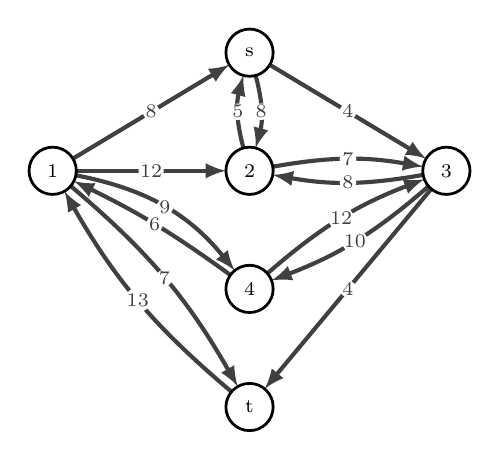
\begin{tikzpicture}[vertex/.style={fill=white}]
                \Vertex[x=2.5,y=1.5,label=s,color=white]{s}
                \Vertex[x=0,y=0,label=1,color=white]{1}
                \Vertex[x=2.5,y=0,label=2,color=white]{2}
                \Vertex[x=5,y=0,label=3,color=white]{3}
                \Vertex[x=2.5,y=-1.5,label=4,color=white]{4}
                \Vertex[x=2.5,y=-3,label=t,color=white]{t}

                \Edge[Direct,bend=15,label=8](s)(2)
                \Edge[Direct,label=4](s)(3)
                \Edge[Direct,label=8](1)(s)
                \Edge[Direct,label=12](1)(2)
                \Edge[Direct,bend=20,label=9](1)(4)
                \Edge[Direct,bend=10,label=7](1)(t)
                \Edge[Direct,bend=15,label=5](2)(s)
                \Edge[Direct,bend=10,label=7](2)(3)
                \Edge[Direct,bend=10,label=8](3)(2)
                \Edge[Direct,bend=10,label=10](3)(4)
                \Edge[Direct,label=4](3)(t)
                \Edge[Direct,bend=-5,label=6](4)(1)
                \Edge[Direct,bend=10,label=12](4)(3)
                \Edge[Direct,bend=10,label=13](t)(1)
            \end{tikzpicture}

            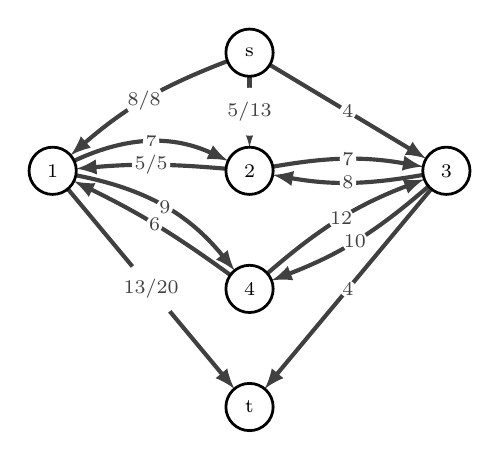
\begin{tikzpicture}[vertex/.style={fill=white}]
                \Vertex[x=2.5,y=1.5,label=s,color=white]{s}
                \Vertex[x=0,y=0,label=1,color=white]{1}
                \Vertex[x=2.5,y=0,label=2,color=white]{2}
                \Vertex[x=5,y=0,label=3,color=white]{3}
                \Vertex[x=2.5,y=-1.5,label=4,color=white]{4}
                \Vertex[x=2.5,y=-3,label=t,color=white]{t}

                \Edge[Direct,bend=-10,label=8/8](s)(1)
                \Edge[Direct,label=5/13](s)(2)
                \Edge[Direct,label=4](s)(3)
                \Edge[Direct,bend=25,label=7](1)(2)
                \Edge[Direct,bend=20,label=9](1)(4)
                \Edge[Direct,label=13/20](1)(t)
                \Edge[Direct,bend=-5,label=5/5](2)(1)
                \Edge[Direct,bend=10,label=7](2)(3)
                \Edge[Direct,bend=10,label=8](3)(2)
                \Edge[Direct,bend=10,label=10](3)(4)
                \Edge[Direct,label=4](3)(t)
                \Edge[Direct,bend=-5,label=6](4)(1)
                \Edge[Direct,bend=10,label=12](4)(3)
            \end{tikzpicture}

            \hrulefill

            Augmenting Path: \(s \rightarrow 2 \rightarrow 3 \rightarrow 4 \rightarrow 1 \rightarrow t\)

            Residue network:

            Flow network:
            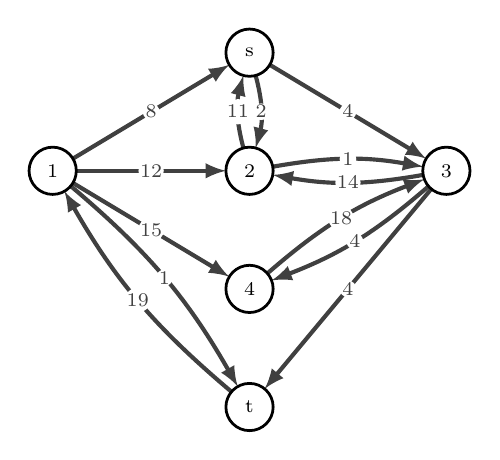
\begin{tikzpicture}[vertex/.style={fill=white}]
                \Vertex[x=2.5,y=1.5,label=s,color=white]{s}
                \Vertex[x=0,y=0,label=1,color=white]{1}
                \Vertex[x=2.5,y=0,label=2,color=white]{2}
                \Vertex[x=5,y=0,label=3,color=white]{3}
                \Vertex[x=2.5,y=-1.5,label=4,color=white]{4}
                \Vertex[x=2.5,y=-3,label=t,color=white]{t}

                \Edge[Direct,bend=15,label=2](s)(2)
                \Edge[Direct,label=4](s)(3)
                \Edge[Direct,label=8](1)(s)
                \Edge[Direct,label=12](1)(2)
                \Edge[Direct,label=15](1)(4)
                \Edge[Direct,bend=10,label=1](1)(t)
                \Edge[Direct,bend=15,label=11](2)(s)
                \Edge[Direct,bend=10,label=1](2)(3)
                \Edge[Direct,bend=10,label=14](3)(2)
                \Edge[Direct,bend=10,label=4](3)(4)
                \Edge[Direct,label=4](3)(t)
                \Edge[Direct,bend=10,label=18](4)(3)
                \Edge[Direct,bend=10,label=19](t)(1)
            \end{tikzpicture}

            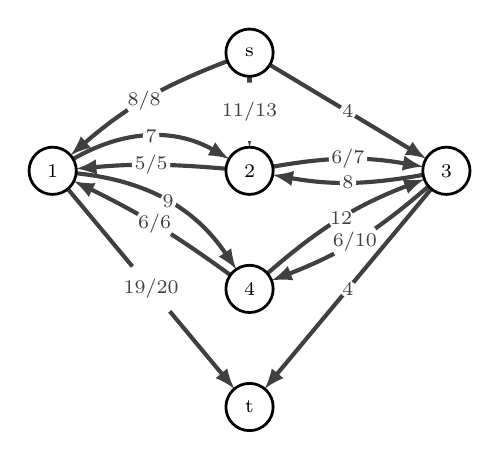
\begin{tikzpicture}[vertex/.style={fill=white}]
                \Vertex[x=2.5,y=1.5,label=s,color=white]{s}
                \Vertex[x=0,y=0,label=1,color=white]{1}
                \Vertex[x=2.5,y=0,label=2,color=white]{2}
                \Vertex[x=5,y=0,label=3,color=white]{3}
                \Vertex[x=2.5,y=-1.5,label=4,color=white]{4}
                \Vertex[x=2.5,y=-3,label=t,color=white]{t}

                \Edge[Direct,bend=-10,label=8/8](s)(1)
                \Edge[Direct,label=11/13](s)(2)
                \Edge[Direct,label=4](s)(3)
                \Edge[Direct,bend=30,label=7](1)(2)
                \Edge[Direct,bend=25,label=9](1)(4)
                \Edge[Direct,label=19/20](1)(t)
                \Edge[Direct,bend=-5,label=5/5](2)(1)
                \Edge[Direct,bend=10,label=6/7](2)(3)
                \Edge[Direct,bend=10,label=8](3)(2)
                \Edge[Direct,bend=10,label=6/10](3)(4)
                \Edge[Direct,label=4](3)(t)
                \Edge[Direct,bend=-5,label=6/6](4)(1)
                \Edge[Direct,bend=10,label=12](4)(3)
            \end{tikzpicture}

            \hrulefill

            Augmenting Path: \(s \rightarrow 3 \rightarrow t\)

            Residue network:

            Flow network:
            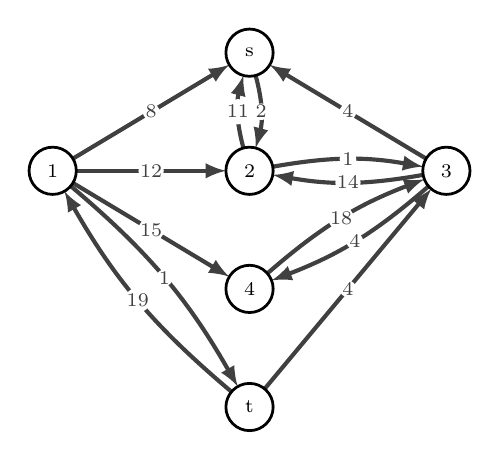
\begin{tikzpicture}[vertex/.style={fill=white}]
                \Vertex[x=2.5,y=1.5,label=s,color=white]{s}
                \Vertex[x=0,y=0,label=1,color=white]{1}
                \Vertex[x=2.5,y=0,label=2,color=white]{2}
                \Vertex[x=5,y=0,label=3,color=white]{3}
                \Vertex[x=2.5,y=-1.5,label=4,color=white]{4}
                \Vertex[x=2.5,y=-3,label=t,color=white]{t}

                \Edge[Direct,bend=15,label=2](s)(2)
                \Edge[Direct,label=8](1)(s)
                \Edge[Direct,label=12](1)(2)
                \Edge[Direct,label=15](1)(4)
                \Edge[Direct,bend=10,label=1](1)(t)
                \Edge[Direct,bend=15,label=11](2)(s)
                \Edge[Direct,bend=10,label=1](2)(3)
                \Edge[Direct,label=4](3)(s)
                \Edge[Direct,bend=10,label=14](3)(2)
                \Edge[Direct,bend=10,label=4](3)(4)
                \Edge[Direct,bend=10,label=18](4)(3)
                \Edge[Direct,bend=10,label=19](t)(1)
                \Edge[Direct,label=4](t)(3)
            \end{tikzpicture}

            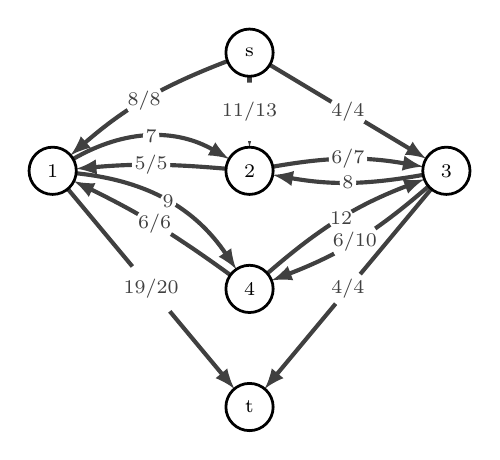
\begin{tikzpicture}[vertex/.style={fill=white}]
                \Vertex[x=2.5,y=1.5,label=s,color=white]{s}
                \Vertex[x=0,y=0,label=1,color=white]{1}
                \Vertex[x=2.5,y=0,label=2,color=white]{2}
                \Vertex[x=5,y=0,label=3,color=white]{3}
                \Vertex[x=2.5,y=-1.5,label=4,color=white]{4}
                \Vertex[x=2.5,y=-3,label=t,color=white]{t}

                \Edge[Direct,bend=-10,label=8/8](s)(1)
                \Edge[Direct,label=11/13](s)(2)
                \Edge[Direct,label=4/4](s)(3)
                \Edge[Direct,bend=30,label=7](1)(2)
                \Edge[Direct,bend=25,label=9](1)(4)
                \Edge[Direct,label=19/20](1)(t)
                \Edge[Direct,bend=-5,label=5/5](2)(1)
                \Edge[Direct,bend=10,label=6/7](2)(3)
                \Edge[Direct,bend=10,label=8](3)(2)
                \Edge[Direct,bend=10,label=6/10](3)(4)
                \Edge[Direct,label=4/4](3)(t)
                \Edge[Direct,bend=-5,label=6/6](4)(1)
                \Edge[Direct,bend=10,label=12](4)(3)
            \end{tikzpicture}

            \hrulefill

            \item
            \begin{align*}
                \text{Max flow}
                    &= f(s,1) + f(s,2) + f(s,3) \\
                    &= 8 + 11 + 4 \\
                    &= 23 \\
                \text{Min cut}
                    &= w(s,1) + w(2,1) + w(4,1) + w(3,t) \\
                    &= 8 + 5 + 6 + 4 \\
                    &= 23
            \end{align*}
        \end{enumerate}

\end{enumerate}

\end{document}